%%%%%%%%%%%%%%%%%%%%%%%%%%%%%%%%%%%%%%%%%
% Programming/Coding Assignment
% LaTeX Template
%
% This template has been downloaded from:
% http://www.latextemplates.com
%
% Original author:
% Ted Pavlic (http://www.tedpavlic.com)
%
% Note:
% The \lipsum[#] commands throughout this template generate dummy text
% to fill the template out. These commands should all be removed when 
% writing assignment content.
%
% This template uses a Perl script as an example snippet of code, most other
% languages are also usable. Configure them in the "CODE INCLUSION 
% CONFIGURATION" section.
%
%%%%%%%%%%%%%%%%%%%%%%%%%%%%%%%%%%%%%%%%%

%----------------------------------------------------------------------------------------
%	PACKAGES AND OTHER DOCUMENT CONFIGURATIONS
%----------------------------------------------------------------------------------------

\documentclass{article}

\usepackage{fancyhdr} % Required for custom headers
\usepackage{lastpage} % Required to determine the last page for the footer
\usepackage{extramarks} % Required for headers and footers
\usepackage[usenames,dvipsnames]{color} % Required for custom colors
\usepackage{graphicx} % Required to insert images
\usepackage{subcaption}
\usepackage{listings} % Required for insertion of code
\usepackage{courier} % Required for the courier font
\usepackage{lipsum} % Used for inserting dummy 'Lorem ipsum' text into the template

% Margins
\topmargin=-0.45in
\evensidemargin=0in
\oddsidemargin=0in
\textwidth=6.5in
\textheight=9.0in
\headsep=0.25in

\linespread{1.1} % Line spacing

% Set up the header and footer
\pagestyle{fancy}
\lhead{\hmwkAuthorName} % Top left header
\chead{\hmwkClass\ (\hmwkClassTime): \hmwkTitle} % Top center head
%\rhead{\firstxmark} % Top right header
\lfoot{\lastxmark} % Bottom left footer
\cfoot{} % Bottom center footer
\rfoot{Page\ \thepage\ of\ \protect\pageref{LastPage}} % Bottom right footer
\renewcommand\headrulewidth{0.4pt} % Size of the header rule
\renewcommand\footrulewidth{0.4pt} % Size of the footer rule

\setlength\parindent{0pt} % Removes all indentation from paragraphs

%----------------------------------------------------------------------------------------
%	CODE INCLUSION CONFIGURATION
%----------------------------------------------------------------------------------------

\definecolor{MyDarkGreen}{rgb}{0.0,0.4,0.0} % This is the color used for comments
\lstloadlanguages{Perl} % Load Perl syntax for listings, for a list of other languages supported see: ftp://ftp.tex.ac.uk/tex-archive/macros/latex/contrib/listings/listings.pdf
\lstset{language=Perl, % Use Perl in this example
        frame=single, % Single frame around code
        basicstyle=\small\ttfamily, % Use small true type font
        keywordstyle=[1]\color{Blue}\bf, % Perl functions bold and blue
        keywordstyle=[2]\color{Purple}, % Perl function arguments purple
        keywordstyle=[3]\color{Blue}\underbar, % Custom functions underlined and blue
        identifierstyle=, % Nothing special about identifiers                                         
        commentstyle=\usefont{T1}{pcr}{m}{sl}\color{MyDarkGreen}\small, % Comments small dark green courier font
        stringstyle=\color{Purple}, % Strings are purple
        showstringspaces=false, % Don't put marks in string spaces
        tabsize=5, % 5 spaces per tab
        %
        % Put standard Perl functions not included in the default language here
        morekeywords={rand},
        %
        % Put Perl function parameters here
        morekeywords=[2]{on, off, interp},
        %
        % Put user defined functions here
        morekeywords=[3]{test},
       	%
        morecomment=[l][\color{Blue}]{...}, % Line continuation (...) like blue comment
        numbers=left, % Line numbers on left
        firstnumber=1, % Line numbers start with line 1
        numberstyle=\tiny\color{Blue}, % Line numbers are blue and small
        stepnumber=5 % Line numbers go in steps of 5
}

% Creates a new command to include a perl script, the first parameter is the filename of the script (without .pl), the second parameter is the caption
\newcommand{\perlscript}[2]{
\begin{itemize}
\item[]\lstinputlisting[caption=#2,label=#1]{#1.pl}
\end{itemize}
}

%----------------------------------------------------------------------------------------
%	DOCUMENT STRUCTURE COMMANDS
%	Skip this unless you know what you're doing
%----------------------------------------------------------------------------------------

% Header and footer for when a page split occurs within a problem environment
\newcommand{\enterProblemHeader}[1]{
%\nobreak\extramarks{#1}{#1 continued on next page\ldots}\nobreak
%\nobreak\extramarks{#1 (continued)}{#1 continued on next page\ldots}\nobreak
}

% Header and footer for when a page split occurs between problem environments
\newcommand{\exitProblemHeader}[1]{
%\nobreak\extramarks{#1 (continued)}{#1 continued on next page\ldots}\nobreak
%\nobreak\extramarks{#1}{}\nobreak
}

\setcounter{secnumdepth}{0} % Removes default section numbers
\newcounter{homeworkProblemCounter} % Creates a counter to keep track of the number of problems
\setcounter{homeworkProblemCounter}{0}

\newcommand{\homeworkProblemName}{}
\newenvironment{homeworkProblem}[1][Part \arabic{homeworkProblemCounter}]{ % Makes a new environment called homeworkProblem which takes 1 argument (custom name) but the default is "Problem #"
\stepcounter{homeworkProblemCounter} % Increase counter for number of problems
\renewcommand{\homeworkProblemName}{#1} % Assign \homeworkProblemName the name of the problem
\section{\homeworkProblemName} % Make a section in the document with the custom problem count
\enterProblemHeader{\homeworkProblemName} % Header and footer within the environment
}{
\exitProblemHeader{\homeworkProblemName} % Header and footer after the environment
}

\newcommand{\problemAnswer}[1]{ % Defines the problem answer command with the content as the only argument
\noindent\framebox[\columnwidth][c]{\begin{minipage}{0.98\columnwidth}#1\end{minipage}} % Makes the box around the problem answer and puts the content inside
}

\newcommand{\homeworkSectionName}{}
\newenvironment{homeworkSection}[1]{ % New environment for sections within homework problems, takes 1 argument - the name of the section
\renewcommand{\homeworkSectionName}{#1} % Assign \homeworkSectionName to the name of the section from the environment argument
\subsection{\homeworkSectionName} % Make a subsection with the custom name of the subsection
\enterProblemHeader{\homeworkProblemName\ [\homeworkSectionName]} % Header and footer within the environment
}{
\enterProblemHeader{\homeworkProblemName} % Header and footer after the environment
}

%----------------------------------------------------------------------------------------
%	NAME AND CLASS SECTION
%----------------------------------------------------------------------------------------

\newcommand{\hmwkTitle}{Project 3} % Assignment title
\newcommand{\hmwkDueDate}{Monday,\ March\ 21,\ 2016} % Due date
\newcommand{\hmwkClass}{CSC321} % Course/class
\newcommand{\hmwkClassTime}{L0101} % Class/lecture time
\newcommand{\hmwkAuthorName}{Mohdhar Noor, Maxwell Huang-Hobbs} % Your name

%----------------------------------------------------------------------------------------
%	TITLE PAGE
%----------------------------------------------------------------------------------------

\title{
\vspace{2in}
\textmd{\textbf{\hmwkClass:\ \hmwkTitle}}\\
\normalsize\vspace{0.1in}\small{Due\ on\ \hmwkDueDate}\\
\vspace{0.1in}
\vspace{3in}
}

\author{\textbf{\hmwkAuthorName} \\ (g3theuma), (g4rbage)}
%\date{} % Insert date here if you want it to appear below your name

%----------------------------------------------------------------------------------------

\begin{document}

\maketitle

\clearpage
%----------------------------------------------------------------------------------------
%	PART 1
%----------------------------------------------------------------------------------------

% To have just one problem per page, simply put a \clearpage after each problem

\begin{homeworkProblem}

\noindent \textit{Classification using single hidden layer neural network}

The images were resized to $32\times 32$ and converted to greyscale. The weights and biases in both layers were initialized to random values generated using \texttt{tf.random\_normal} a Guassian distribution with a mean of 0 and a standard deviation of 0.01. The activation function used in the hidden layer was $tanh$. We used a fully connected network with a flattened 784 element vector denoting an image, a 300 unit hidden layer and 6 element one-hot enconding for a output, as was done in project 2. The learning rate is shown in Figure~\ref{fig:lrp1}. The final learning rates for the network were 0.87 for the training set, 0.80 for the validation set and 0.77 for the test set.


\begin{figure*}[h!]
    \centering
    \includegraphics[scale=0.5]{p1/learning_rate.png}
    \caption{learning rate of a single hidden layer network}
    \label{fig:lrp1}
\end{figure*}

\end{homeworkProblem}
\clearpage
%----------------------------------------------------------------------------------------
%	PART 2
%----------------------------------------------------------------------------------------

\begin{homeworkProblem}
\noindent \textit{Classification using the Colvolutional layers of Alexnet}

In order to use the provided alexnet implementation, a new dataset of colored 227*227 RGB images was scraped. The provided alexnet weights were used as constants in the network, and fed into a fully connected neural network.

This is the same as running alexnet up to conv4 on the input data, recording the output, and feeding the information into a fully connected network.

The fully connected layer was initialized with random weights and biases, distributed using a Gaussian distribution with $\sigma=0.001$. Gradient descent was performed with a learning rate of 0.005.

In order to shorten computation time, the network's performance was evaluated once every 100 generations. (x scale in 100s of generations)

\begin{figure*}[h!]
    \centering
    \includegraphics[scale=0.5]{p2/learning_rate.png}
    \caption{learning rate of the neural network. }
    \label{fig:lrp1}
\end{figure*}

The neural network seems to level out at about $30\%$ accuracy at classification. This suggests that the network was poorly initialized and the network becae trapped in a local optima. 

Likely this could have been fixed by increasing the batch size that the network learned on. The provided alexnet implementation could not batch process inputs, and due to time constraints we did not implement it ourselves, and so were forced to train with a batch size of 1.

\end{homeworkProblem}
\clearpage
%----------------------------------------------------------------------------------------
%	PROBLEM 3
%----------------------------------------------------------------------------------------

\begin{homeworkProblem}
\noindent \textit{Visualizing Hidden Weights.}

The weights used was the weight matrix connecting the features to the hidden layer ('hiddden weights'). The hidden weights for the 300 unit hidden network display discernable components of an actor's face such as the brows, nose, mouth, hairline and jaw while the 800 unit weights do not exhibit that level of detail.

\begin{figure*}[!ht]
\centering
\begin{subfigure}{.35\textwidth}
  
\includegraphics[width=.80\linewidth]{p3/300_0199.png}
  \caption{Example feature from the \\ 300-hidden network.}
  \label{fig:sfig1}
\end{subfigure}
\begin{subfigure}{.35\textwidth}
  
\includegraphics[width=.80\linewidth]{p3/300_0246.png}
  \caption{Example feature from the \\ 300-hidden network.}
  \label{fig:sfig2}
\end{subfigure}\\
\begin{subfigure}{.35\textwidth}
  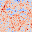
\includegraphics[width=.80\linewidth]{p3/800_0412.png}
  \caption{Example feature from the \\ 800-hidden network.}
  \label{fig:sfig3}
\end{subfigure}
\begin{subfigure}{.35\textwidth}
  
\includegraphics[width=.80\linewidth]{p3/800_0691.png}
  \caption{Example feature from the \\ 800-hidden network.}
  \label{fig:sfig4}
\end{subfigure}
\caption{}
\label{fig:pcs}
\end{figure*}

Figure~\ref{fig:pcs} Shows examples of features in the hidden layer of the 300 and 800 layer neural networks. They seem to be selecting strongly for certain facial features and against specific placements of other facial features. 

For example, figure ~\ref{fig:sfig2} appears to be selecting towards a particluar placement of the eyes and against a specific relative positioning of the nose. This might suggest that some actors / actresses in the dataset can be distinguished by the relative position of their eyes and nose.

\end{homeworkProblem}
\clearpage

%----------------------------------------------------------------------------------------
%	Part 4
%----------------------------------------------------------------------------------------

\begin{homeworkProblem}
\noindent \textit{Classification using AlexNet}

Our implementation of part 2 covers the requirements for part 4 (the AlexNet input layers up to conv4 are implemented as constants, and the fully connected layer is trained on the output of part conv4).


AlexNet's layers from conv1-conv4 were fixed as constants using the provided weights, and a fully connected network was added from the conv4 output to the output of the network.



\begin{figure*}[!ht]
\centering
\begin{subfigure}{.35\textwidth}
  \includegraphics[width=.80\linewidth]{p4/1433.png}
  \label{fig:sfig1}
\end{subfigure}
\begin{subfigure}{.35\textwidth}
    Network Output: $1$ \\
    (Gerard Butler)
\end{subfigure}
\caption{Example of the neural network classifying a face correctly}
\label{fig:pcs}
\end{figure*}


\begin{figure*}[!ht]
\centering
\begin{subfigure}{.35\textwidth}
  \includegraphics[width=.80\linewidth]{p4/1559.png}
  \label{fig:sfig1}
\end{subfigure}
\begin{subfigure}{.35\textwidth}
    Network Output: $1$ \\
    (Lorraine Braco)
\end{subfigure}
\caption{Example of the neural network classifying a face incorrectly}
\label{fig:pcs}
\end{figure*}



\end{homeworkProblem}
\clearpage


%----------------------------------------------------------------------------------------
%	Part 5
%----------------------------------------------------------------------------------------

\begin{homeworkProblem}
\noindent \textit{Gradients of the input layer}

The gradient of the softmaxed output of the network with respect to any input was consistently 0, i.e. all the neurons on the input layer are dead.


\begin{figure*}[!ht]
\centering
\begin{subfigure}{.35\textwidth}
  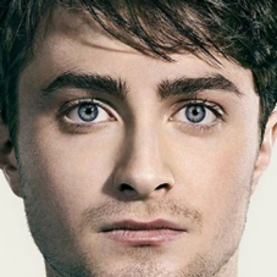
\includegraphics[width=.80\linewidth]{p5/861.png}
  \label{fig:sfig1}
\end{subfigure}
\begin{subfigure}{.35\textwidth}
  \includegraphics[width=.80\linewidth]{p5/radcliffe_init.png}
  \label{fig:sfig1}
\end{subfigure}
\caption{Gradient of output likelihoods wrt input image}
\label{fig:pcs}
\end{figure*}


When the gradient of the non-softmaxed output is visualized, It gives images of noise with smooth areas around edges of the image, with what appear to be diamond patterns over most of the image

Its possible this is from the network memorizing features of the training set and using these as the criteria to decide between classes.

\begin{figure*}[!ht]
\centering
\begin{subfigure}{.35\textwidth}
  \includegraphics[width=.80\linewidth]{p5/1003.png}
  \label{fig:sfig1}
\end{subfigure}
\begin{subfigure}{.35\textwidth}
  \includegraphics[width=.80\linewidth]{p5/1003_radcliffe_grad.png}
  \label{fig:sfig1}
\end{subfigure}
\begin{subfigure}{.35\textwidth}
  \includegraphics[width=.80\linewidth]{p5/1007.png}
  \label{fig:sfig1}
\end{subfigure}
\begin{subfigure}{.35\textwidth}
  \includegraphics[width=.80\linewidth]{p5/1007_radcliffe_grad.png}
  \label{fig:sfig1}
\end{subfigure}
\caption{Gradient of output wrt input image}
\label{fig:pcs}
\end{figure*}


\end{homeworkProblem}
\clearpage

\end{document}